\chapter{Cheatsheet}

% Formato de texto
\textbf{Negrita}, \textit{Itálica}, \underline{Subrayado}  

% Listas
\begin{itemize}
    \item Primer ítem
    \item Segundo ítem
\end{itemize}

\begin{enumerate}
    \item Ítem 1
    \item Ítem 2
\end{enumerate}

% Ecuaciones
Ecuación en la misma línea: $a^2 + b^2 = c^2$

Ecuación en medio: $$E = mc^2$$

% Figuras
\begin{figure}[htbp]
    \centering
    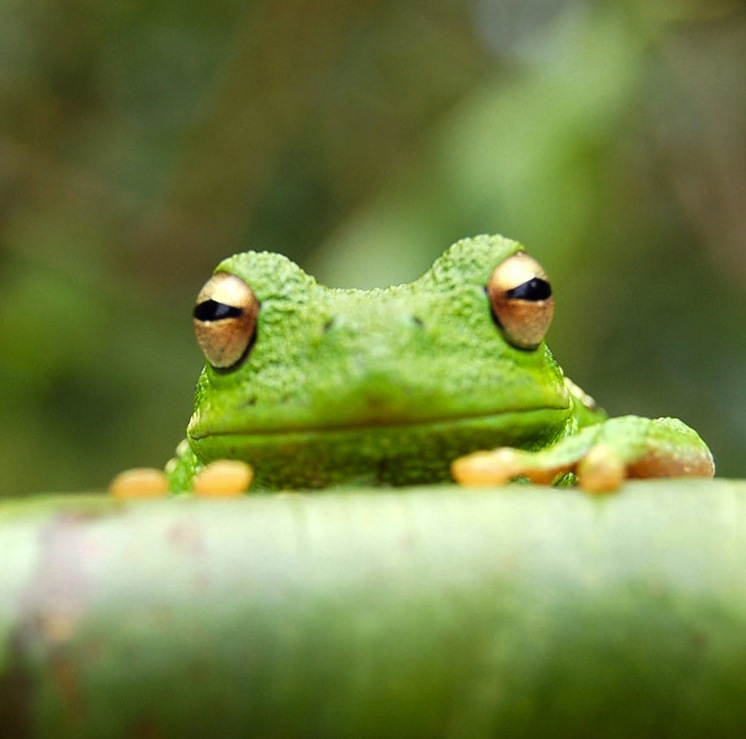
\includegraphics[width=0.3\linewidth]{figuras/frog.jpg}
    \caption{Ejemplo de cómo presentar una ilustración utilizando una foto del monumento a la brigada del Negev}
    \label{fig:ejemplo}
    \sourcefig{Israel Tour Guides}{2013}{https://israel-tourguide.info/2013/04/20/photo-of-the-week-negev-brigade-monument}
\end{figure}

% Tablas
\begin{table}[htbp]
    \centering
    \caption{Tabla de ejemplo}
    \begin{tabular}{|c|c|c|}
    \hline
    A & B & C \\ \hline
    1 & 2 & 3 \\ \hline
    4 & 5 & 6 \\ \hline
    \end{tabular}
    \label{tab:ejemplo}
\end{table}

% Referencias cruzadas
Ver Figura \ref{fig:ejemplo} y Tabla \ref{tab:ejemplo}.

% Citas y bibliografía
Ejemplo de cita: \cite{dinosaurios2006}; \parencite{dinosaurios2006}

% Enlaces
Ejemplo de enlace: \href{https://www.overleaf.com}{Overleaf}

Ejemplo de url: \url{https://www.overleaf.com}

% Código
\begin{lstlisting}[language=Python, caption=Hola Mundo en Python]
def saludo():
    print("Hola, mundo!")

saludo()
\end{lstlisting}

\begin{sloppypar}
    Palabras monoespaciadas: El directorio \code{\%HOME} se encuentra en \code{/home/<usuario>}
\end{sloppypar}
